\chapter{スタートプロジェクトの作成}
\label{chap:02-create-react-app}
\begin{starterabstract}
  本章では、「create{-}react{-}app」と言う、reactアプリケーションのひな型がコマンドひとつで作成できる優れものを使用して、
スタート用のアプリケーションを作成し、ブラウザで表示するまでを行います。

 また、作成するプロジェクトは、TypesScriptを使用します。コード記法の指摘・修正を行えるよう「eslint」、「prettier」の設定も行います。

\end{starterabstract}

\section{create{-}react{-}appコマンド}
\keeplastskip{
  \label{sec:2-1}
  \label{sec-01command}
  \par\nobreak
}

Reactアプリケーションをゼロから作成するためには、\\[0pt]
\\[0pt]
* 「nodeプロジェクト」に必要なpackage.jsonを作成
* reactなど必要なライブラリのインストール
* 作成したアプリケーションが、古いブラウザでも実行できるようにコードを変換(Babel使用)
* 出力するファイルをまとめる(バンドルする {-} webpack使用)

など、reactライブラリのインストール以外にも、Babelやwebpackをインストールして設定ファイルを作成しなくてはなりません。

また、使用するライブラリによっては、Babelのプラグインのインストールや設定など、アプリケーションのコードを書き始める前の作業がたいへんです。

しかし、「そんなメンドウなことは、やってられない。」と誰しもが思ったか、
すぐにでもコードを書き始めることのできるスタート用アプリケーションが、react開発元のFacebookから提供されています。

さらに、そのスタート用アプリケーションは、コマンド一発でインストールできます。

ターミナルを起動し、プロジェクトフォルダを作成するフォルダへ移動します。

\def\startercodeblockfontsize{}
\begin{starterterminal}[]{create{-}react{-}appでスタート用アプリケーション作成}\seqsplit{  \textdollar{} \textgreater{} npx create react{-}app プロジェクト名 {-}{-}template typescript}\end{starterterminal}

で、「プロジェクト名」のフォルダが作成され、スグにでも開発に取りかかれます。

\def\startercodeblockfontsize{}
\begin{starterterminal}[]{}\seqsplit{  Success! Created yourproject at yourproject\textunderscore{}path
  Inside that directory, you can run several commands:

    yarn start
      Starts the development server.

    yarn build
      Bundles the app into static files for production.

    yarn test
      Starts the test runner.

    yarn eject
      Removes this tool and copies build dependencies, configuration files
      and scripts into the app directory. If you do this, you can’t go back!

  We suggest that you begin by typing:

    cd yourproject
    yarn start

  Happy hacking!}\end{starterterminal}

で、プロジェクト作成が完了します。

\begin{starterquote}

コンソールには、Facebookが関わっているノード・パッケージマネージャーの「yarn」を使ったコマンドが表示されています。

\begin{description}
\item[yarn start] \mbox{} \\
開発用サーバの開始。
\item[yarn build] \mbox{} \\
製品用に静的はファイルにアプリケーションをまとめる。
\item[yarn test] \mbox{} \\
テストランナーの開始。
\item[yarn eject] \mbox{} \\
ツール(create{-}react{-}app)を取り除き、依存関係、設定ファイル、スクリプトをappディレクトリにコピーする。
\end{description}

 と、あります。

 yarnは、pnp(プラグ&プレイ{-}依存関係(node\textunderscore{}modulesフォルダ以下にインストールされるパッケージ)を仮想化してロードする機能)を
導入したv2で大きく変わっています。今ではv3もリリースされています。

PnPなしでもyarn v3を使うこともできるようですが、私はnpm(ノード・パッケージマネージャー)を使っています。

\end{starterquote}
\begin{starternote}[]{github}

ここまでの作業は、GitHubにあります。
\textless{}!{-}{-} textlint{-}disable {-}{-}\textgreater{}

\def\startercodeblockfontsize{}
\begin{starterterminal}[]{GitHubから}\seqsplit{    \textdollar{} \textgreater{} git clone {-}b 00\textunderscore{}create{-}react{-}app https://github.com/yaruo{-}react{-}redux/yaruo{-}blog.git}\end{starterterminal}

\textless{}!{-}{-} textlit{-}enable {-}{-}\textgreater{}

\end{starternote}

\section{アプリケーションを実行}
\keeplastskip{
  \label{sec:2-2}
  \label{sec-02yarnstart}
  \par\nobreak
}

アプリケーションが作成できましたので、実行してみます。

ターミナルに表示されているように、プロジェクトフォルダへ移動し、スタート用のコマンドを入力します。

\def\startercodeblockfontsize{}
\begin{starterterminal}[]{}\seqsplit{  \textdollar{} \textgreater{} cd プロジェクト名
  \textdollar{} \textgreater{} npm start}\end{starterterminal}

すると、webpackに同梱されている開発用のweb serverが起動し、デフォルトでは、port:3000でアプリケーションへアクセスできます。

\def\startercodeblockfontsize{}
\begin{starterterminal}[]{}\seqsplit{Compiled successfully!

You can now view yourproject in the browser.

  Local:            http://localhost:3000
  On Your Network:  http://pcのローカルIPアドレス:3000

Note that the development build is not optimized.
To create a production build, use yarn build.}\end{starterterminal}

Google Chromeが起動し、http://localhost:3000へアクセスし以下のページが表示されます。

\begin{reviewimage}[H]%%02_cra_start
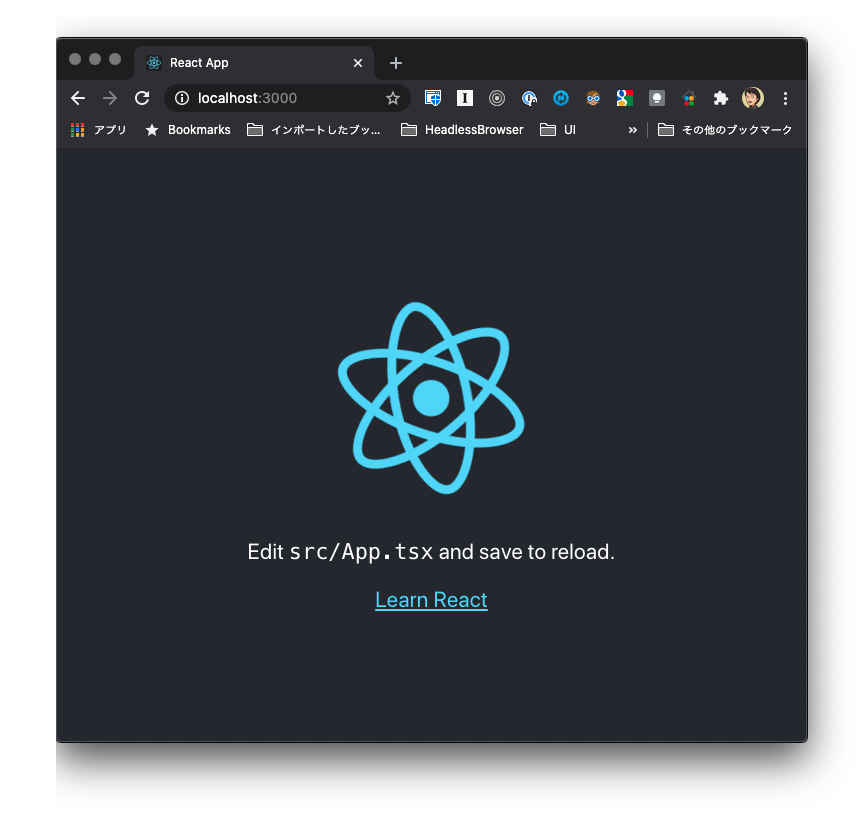
\includegraphics[width=1.0\maxwidth]{./images/02-create-react-app/02_cra_start.png}%
\reviewimagecaption{create{-}react{-}appの画面}
\label{image:02-create-react-app:02_cra_start}
\end{reviewimage}

このページが表示されれば成功です。

\section{create{-}react{-}appで作成された中身}
\keeplastskip{
  \label{sec:2-3}
  \label{sec-03cra-desc}
  \par\nobreak
}

create{-}react{-}appで作成された中身は、以下となります(使用するテンプレートにより作成されるファイル・フォルダは異なる)。

\def\startercodeblockfontsize{}
\begin{starterterminal}[]{package.json}\seqsplit{  .
  ├── node\textunderscore{}modules
  ├── README.md
  ├── package.json
  ├── public
  │   ├── favicon.ico
  │   ├── index.html
  │   ├── logo192.png
  │   ├── logo512.png
  │   ├── manifest.json
  │   └── robots.txt
  ├── src
  │   ├── App.css
  │   ├── App.test.tsx
  │   ├── App.tsx
  │   ├── index.css
  │   ├── index.tsx
  │   ├── logo.svg
  │   ├── react{-}app{-}env.d.ts
  │   ├── reportWebVitals.ts
  │   └── setupTests.ts
  ├── tsconfig.json
  └── yarn.lock}\end{starterterminal}

package.jsonファイルは、Node.jsを使用するプロジェクトの設計図にあたるものです。
\\[0pt]
Node.jsを使うプロジェクトを開始する場合には、プロジェクトフォルダで「npm init」を行うと対話形式で「package.json」を作成しますが、
create{-}react{-}appコマンドを使用すると、package.jsonも以下のように作成されます。

\def\startercodeblockfontsize{}
\begin{starterprogram}[]{package.json}\seqsplit{  \{
    "name": "yaruo{-}blog",
    "version": "0.1.0",
    "private": true,
    "dependencies": \{
      "@testing{-}library/jest{-}dom": "\textasciicircum{}5.11.4",
      "@testing{-}library/react": "\textasciicircum{}11.1.0",
      "@testing{-}library/user{-}event": "\textasciicircum{}12.1.10",
      "@types/jest": "\textasciicircum{}26.0.15",
      "@types/node": "\textasciicircum{}12.0.0",
      "@types/react": "\textasciicircum{}17.0.0",
      "@types/react{-}dom": "\textasciicircum{}17.0.0",
      "react": "\textasciicircum{}17.0.2",
      "react{-}dom": "\textasciicircum{}17.0.2",
      "react{-}scripts": "4.0.3",
      "typescript": "\textasciicircum{}4.1.2",
      "web{-}vitals": "\textasciicircum{}1.0.1"
    \},
    "scripts": \{
      "start": "react{-}scripts start",
      "build": "react{-}scripts build",
      "test": "react{-}scripts test",
      "eject": "react{-}scripts eject"
    \},
    "eslintConfig": \{
      "extends": [
        "react{-}app",
        "react{-}app/jest"
      ]
    \},
    "browserslist": \{
      "production": [
        "\textgreater{}0.2\%",
        "not dead",
        "not op\textunderscore{}mini all"
      ],
      "development": [
        "last 1 chrome version",
        "last 1 firefox version",
        "last 1 safari version"
      ]
    \}
  \}}\end{starterprogram}

package.json内にある「scripts」にあるものがコマンドになります。react{-}scriptsは、npmスクリプトを連続、または、並列に実行してくれるものです。
\\[0pt]

package.jsonの「dependencies」には、実行に必要でインストール済みのnpmパッケージが記載されています。
必要なnpmパッケージをインストールすると、ここに自動的に追記されます。
\\[0pt]
また、開発時のみ必要なパッケージ(buildしたときには組み込まれない)は、「devDependencies」に追加されます。
\\[0pt]

\section{eslint、prettier}
\keeplastskip{
  \label{sec:2-4}
  \label{sec-03lint}
  \par\nobreak
}

「lint」は、C言語用のコンパイラよりも詳細で厳密なチェックを行うプログラムです。
コンパイル前にコードをチェックするために使われます。

それが、いつしかコードをチェック・解析することを「lint」、lintを行うプログラムをlinterと呼ぶようになったそうです。

JavaScript(ECMAScript)用のlinterが、「eslint」になります。もちろん、Java、HTML、Pythonなどにもlinterがあります。

「eslint」は、JavaScriptで指定されたルールと違うコードの書き方をしている部分を指摘してくれます。
その指定されたルールとは、たいていの場合にはJavaScriptに詳しい人達が決めたもので、良く使われるものは、かの有名なAirBnBの開発チームのものです。

もちろん、ルールは改変・追加もできます。

チェックしてくれるのは、たとえば、\\[0pt]

\begin{starteritemize}
\item constで宣言している変数への代入
\item 未定義の変数やモジュールの使用
\item 分割代入の使用を推奨
\end{starteritemize}

などがありますが、何をチェックし指摘するのかは、チーム毎、プロジェクト毎に自由に決めることができます。

「prettier」は、コードを整形(インデント、改行など)してくれるツールです。
実は、eslintでもコード整形はできるのですが、コード整形はprettierの方が優れいます。

そのために、\\[0pt]

\begin{starteritemize}
\item コードチェックは、eslint
\item コード整形は、prettier
\end{starteritemize}

と、得意なものに任せます。
\\[0pt]

この便利な機能こそが、第1章で紹介した\\[0pt]

\begin{starteritemize}
\item Eslint
\item Prettier
\end{starteritemize}

になります。
\\[0pt]

\subsection{eslint、prettierのインストール}
\keeplastskip{
  \label{sec:2-4-1}
  \label{sec-03eslint}
  \par\nobreak
}

create{-}react{-}appを使用して作成したスタートアッププロジェクトには、eslintは導入済みですので設定し直し、必要な関連パッケージをインストールします。

ターミナルに以下のように「eslint {-}{-}init」と初期化コマンドを入力します。

\def\startercodeblockfontsize{}
\begin{starterterminal}[]{eslintの初期化}\seqsplit{  \textdollar{} npx eslint {-}{-}init}\end{starterterminal}

「?」が行頭にある質問と選択枝が表示されますので、カーソルキーで選択枝を選びエンターキーで次ぎの質問に移ります。

\def\startercodeblockfontsize{}
\begin{starterterminal}[]{eslintの質問に答える}\seqsplit{  ? How would you like to use ESLint? …
  ❯ To check syntax only            {\reviewballoon{選択したものに > が表示される}}
    To check syntax and find problems
    To check syntax, find problems, and enforce code style}\end{starterterminal}

最後の質問に答えると必要なパッケージをインストールするか尋ねられますので「Yes」と答えてます。

\def\startercodeblockfontsize{}
\begin{starterterminal}[]{eslintへの答え}\seqsplit{  ✔ How would you like to use ESLint? · syntax
  ✔ What type of modules does your project use? · esm
  ✔ Which framework does your project use? · react
  ✔ Does your project use TypeScript? · No / Yes    {\reviewballoon{Yesを選択}}
  ✔ Where does your code run? · browser
  ✔ What format do you want your config file to be in? · JavaScript
  Local ESLint installation not found.
  The config that you've selected requires the following dependencies:

  eslint{-}plugin{-}react@latest @typescript{-}eslint/eslint{-}plugin@latest @typescript{-}eslint/parser@latest eslint@latest
  ✔ Would you like to install them now with npm? · No / Yes}\end{starterterminal}
\def\startercodeblockfontsize{}
\begin{starterprogram}[]{package.jsonにeslint関連のパッケージがインストールされました。}\seqsplit{  "devDependencies": \{
    "@typescript{-}eslint/eslint{-}plugin": "\textasciicircum{}5.4.0",
    "@typescript{-}eslint/parser": "\textasciicircum{}5.4.0",
    "eslint": "\textasciicircum{}8.2.0",
    "eslint{-}plugin{-}react": "\textasciicircum{}7.27.0"
  \}}\end{starterprogram}

また、eslintの設定ファイル「.eslintrc.js」が作成されています。

\def\startercodeblockfontsize{}
\begin{starterprogram}[]{.eslint.js}\seqsplit{  module.exports = \{
      "env": \{
          "browser": true,
          "es2021": true
      \},
      "extends": "plugin:react/recommended",
      "parser": "@typescript{-}eslint/parser",
      "parserOptions": \{
          "ecmaFeatures": \{
              "jsx": true
          \},
          "ecmaVersion": 12,
          "sourceType": "module"
      \},
      "plugins": [
          "react",
          "@typescript{-}eslint"
      ],
      "rules": \{
      \}
  \};}\end{starterprogram}

設定ファイル「.eslint.js」で、どのようなルールが適用されるのかを確認します。
適用されるルールが、「current\textunderscore{}rules.txt」に書き出されます。

\def\startercodeblockfontsize{}
\begin{starterterminal}[]{eslint設定で適用されるルール}\seqsplit{ \textdollar{} npx eslint {-}{-}print{-}config .eslint.js \textgreater{} current\textunderscore{}rules.txt}\end{starterterminal}

eslintで使用するルールは一般的なものをベースにしたいので、あのairbnbのルールをインストールします。

\def\startercodeblockfontsize{}
\begin{starterterminal}[]{airbnbのルーツのインストール}\seqsplit{ \textdollar{}  npx install{-}peerdeps {-}{-}dev eslint{-}config{-}airbnb
    install{-}peerdeps v3.0.3
    It seems as if you are using Yarn.
    Would you like to use Yarn for the installation? (y/n) n{\reviewballoon{yarnを使っているのか聞かれるので、noである「n」を入力}}}\end{starterterminal}

airbnbのルールをインストールしたので、設定ファイルに追加します。

\def\startercodeblockfontsize{}
\begin{starterprogram}[]{.eslint.jsへairbnbルールを適用}\seqsplit{  "extends": [
      "plugin:react/recommended",
      "airbnb",     {\reviewballoon{airbnbのルール}}
      "airbnb/hooks", {\reviewballoon{airbnbのReact hooksのルール}}
  ],}\end{starterprogram}

再度、ルールを出力すると適用されるルールがずいぶん増えているのが分かります。
\\[0pt]
\\[0pt]
次に、TypeScriptもチェックできるようにルールを追加します。「plugin:」の4行を追加しました。

\def\startercodeblockfontsize{}
\begin{starterprogram}[]{.eslint.jsのextends部分}\seqsplit{  "extends": [
      "plugin:react/recommended",
      "airbnb",
      "airbnb/hooks",
      "plugin:@typescript{-}eslint/recommended",
      "plugin:@typescript{-}eslint/recommended{-}requiring{-}type{-}checking",
      "plugin:import/recommended",
      "plugin:import/typescript",
  ],}\end{starterprogram}

TypeScript用ルールを追加しましたので、「parserOptions」を以下のように変更する。

\def\startercodeblockfontsize{}
\begin{starterprogram}[]{.eslint.jsのparserOptions部分}\seqsplit{  "parserOptions": \{
    "ecmaFeatures": \{
        "jsx": true
    \},
    "ecmaVersion": 12,
    "sourceType": "module",
    "tsconfigRootDir": \textunderscore{}\textunderscore{}dirname,
    "project": ["./tsconfig.json"],
  \},}\end{starterprogram}

これでルールの適用は完了したが、都合の悪いルールは設定ファイルにてルールの上書をする。

\def\startercodeblockfontsize{}
\begin{starterprogram}[]{.eslint.jsのrulesへ追加}\seqsplit{  "rules": \{
      "import/extensions": [
          "error",
          \{
            js: "never",
            jsx: "never",
            ts: "never",
            tsx: "never",
          \},
        ],
        "react/jsx{-}filename{-}extension": [
          "error",
          \{
            extensions: [".jsx", ".tsx"],
          \},
        ],
        "react/react{-}in{-}jsx{-}scope": "off",
        "no{-}void": [
          "error",
          \{
            allowAsStatement: true,
          \},
        ],
  \}}\end{starterprogram}

ここからは、Prettierのインストールと設定する。

\def\startercodeblockfontsize{}
\begin{starterterminal}[]{Prettierのインストール}\seqsplit{  \textdollar{} npm install {-}D prettier eslint{-}config{-}prettier}\end{starterterminal}

インストールが完了すると、package.jsonに追加されます。

\def\startercodeblockfontsize{}
\begin{starterprogram}[]{package.json}\seqsplit{  "devDependencies": \{
    "@typescript{-}eslint/eslint{-}plugin": "\textasciicircum{}5.4.0",
    "@typescript{-}eslint/parser": "\textasciicircum{}5.4.0",
    "eslint": "\textasciicircum{}8.2.0",
    "eslint{-}config{-}airbnb": "\textasciicircum{}19.0.0",
    "eslint{-}config{-}prettier": "\textasciicircum{}8.3.0",
    "eslint{-}plugin{-}import": "\textasciicircum{}2.25.3",
    "eslint{-}plugin{-}jsx{-}a11y": "\textasciicircum{}6.5.1",
    "eslint{-}plugin{-}react": "\textasciicircum{}7.27.0",
    "eslint{-}plugin{-}react{-}hooks": "\textasciicircum{}4.3.0",
    "prettier": "\textasciicircum{}2.4.1"
  \}}\end{starterprogram}

Pretterのチェックを「.eslint.js」へ追加します。

\def\startercodeblockfontsize{}
\begin{starterprogram}[]{.eslint.js}\seqsplit{  "extends": [
      "plugin:react/recommended",
      "airbnb",
      "airbnb/hooks",
      "plugin:@typescript{-}eslint/recommended",
      "plugin:@typescript{-}eslint/recommended{-}requiring{-}type{-}checking",
      "plugin:import/recommended",
      "plugin:import/typescript",
      "prettier",   {\reviewballoon{prettierを追加}}
  ],}\end{starterprogram}

pritterの設定ファイル「.prettierrc」を追加します。設定可能なオプションは、
Prettierオプション\footnote{\url{https://prettier.io/docs/en/options.html}}で確認できます。

ほぼすべてがデフォルトでも良いのですが、create{-}react{-}appがシングルクオートなので設定します。

\def\startercodeblockfontsize{}
\begin{starterprogram}[]{.prettierrc}\seqsplit{  \{
    "singleQuote": true
  \}}\end{starterprogram}

eslintとprettierが衝突すると検出・修正ループに入りますので、チェックします。

\def\startercodeblockfontsize{}
\begin{starterterminal}[]{eslint、prettierの衝突検出}\seqsplit{  \textdollar{} npx eslint{-}config{-}prettier 'src/**/*.\{js,jsx,ts,tsx\}'
    No rules that are unnecessary or conflict with Prettier were found.}\end{starterterminal}

無事に衝突なしとなりました。

package.jsonにチェック用のスクリプトコマンドを追加します。

\def\startercodeblockfontsize{}
\begin{starterprogram}[]{package.json}\seqsplit{  "scripts": \{
    "start": "react{-}scripts start",
    "build": "react{-}scripts build",
    "test": "react{-}scripts test",
    "lint": "eslint 'src/**/*.\{js,jsx,ts,tsx\}'", {\reviewballoon{eslint用コマンドを追加}}
    "eject": "react{-}scripts eject"
  \},}\end{starterprogram}

Eslint、Prettierの設定が完了しましたので、srcフォルダにある「App.tsx」を開いてみると、
ルールから外れるものは指摘されています。

\begin{reviewimage}[H]%%03_eslint_prettier
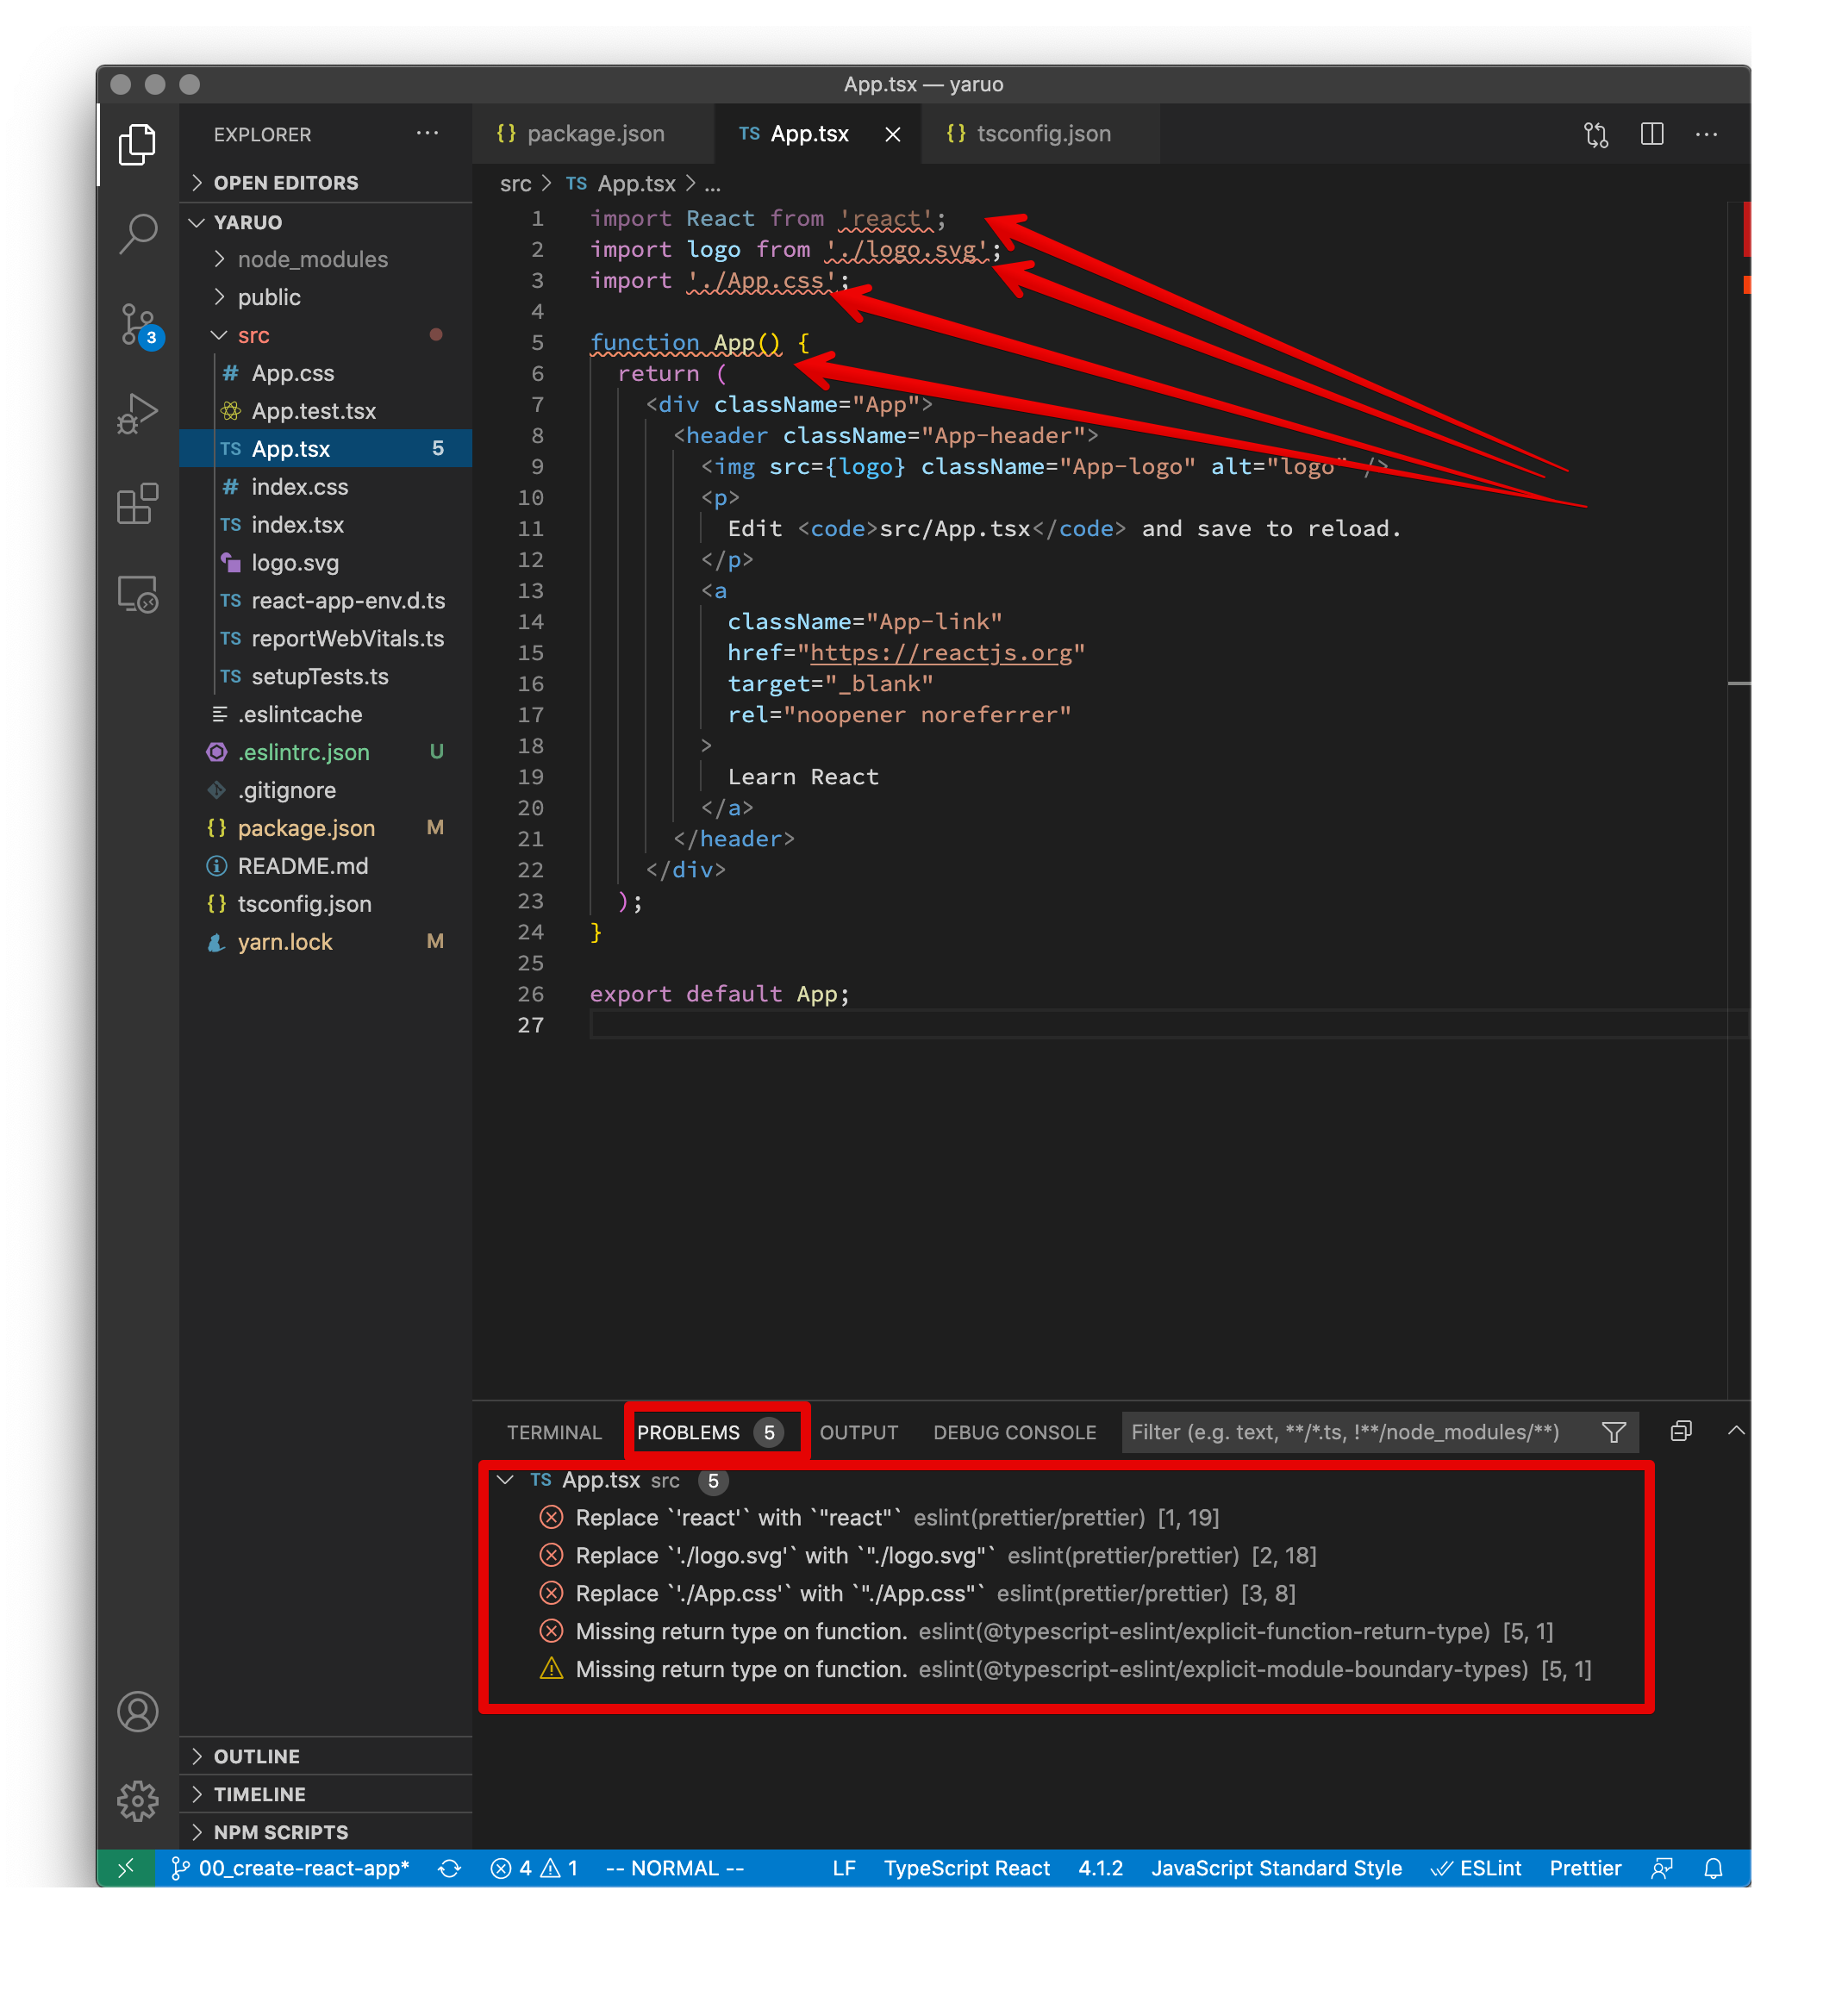
\includegraphics[width=1.0\maxwidth]{./images/02-create-react-app/03_eslint_prettier.png}%
\reviewimagecaption{Eslint、Prettierに怒られてます}
\label{image:02-create-react-app:03_eslint_prettier}
\end{reviewimage}

\section{eslint、prettierの指摘を修正}
\keeplastskip{
  \label{sec:2-5}
  \label{sec-04fix}
  \par\nobreak
}

ESlint、Prettierは指摘するだけではなく、修正案の提示・修正(できるものだけですが...)までしてくれます。

VSCodeにPrettier拡張機能を追加してあれば、
以下のように、VSCode側で設定すると、ファイルを保存する度に自動で修正をいれることもできます。

私は、修正を自分のタイミングで行いたいのでVSCode側の設定は行っていません。

もし、VSCode側の設定をする場合には、VSCodeで\\[0pt]
[File]{-}\textgreater{}[Preferences]{-}\textgreater{}[Settings]にて、以下の各項目を検索して設定するか、settings.jsonへ追加してください。

\def\startercodeblockfontsize{}
\begin{starterprogram}[]{VSCodeの設定}\seqsplit{"editor.formatOnSave": true,
"[JavaScript]": \{
  "editor.formatOnSave": false
\},
"[JavaScriptreact]": \{
  "editor.formatOnSave": false
\},
"[typescript]": \{
  "editor.formatOnSave": false
\},
"[typescriptreact]": \{
  "editor.formatOnSave": false
\},
"editor.codeActionsOnSave": \{
    "source.fixAll": true,
    "source.fixAll.eslint": false
\},
"prettier.disableLanguages": ["JavaScript", "JavaScriptreact", "typescript", "typescriptreact"],}\end{starterprogram}

VSCode上で、\\[0pt]

\begin{starteritemize}
\item 赤波線で指摘されている
\item 問題タブに表示されている
\end{starteritemize}

ものを修正します。

App.tsxの赤波線の上にマウスポンタを置くとeslintのコード、この場合は「no{-}use{-}before{-}define」が表示されます。、
さらに、「コマンドキー(Windowsでは、ctrl) + ピリオド」を押すと、修正方法が提示されます。

「Fix all auto{-}fixable problems」を選択すると、自動修復可能なものを修正してくれます。

\begin{reviewimage}[H]%%04_eslint_prettier_fix
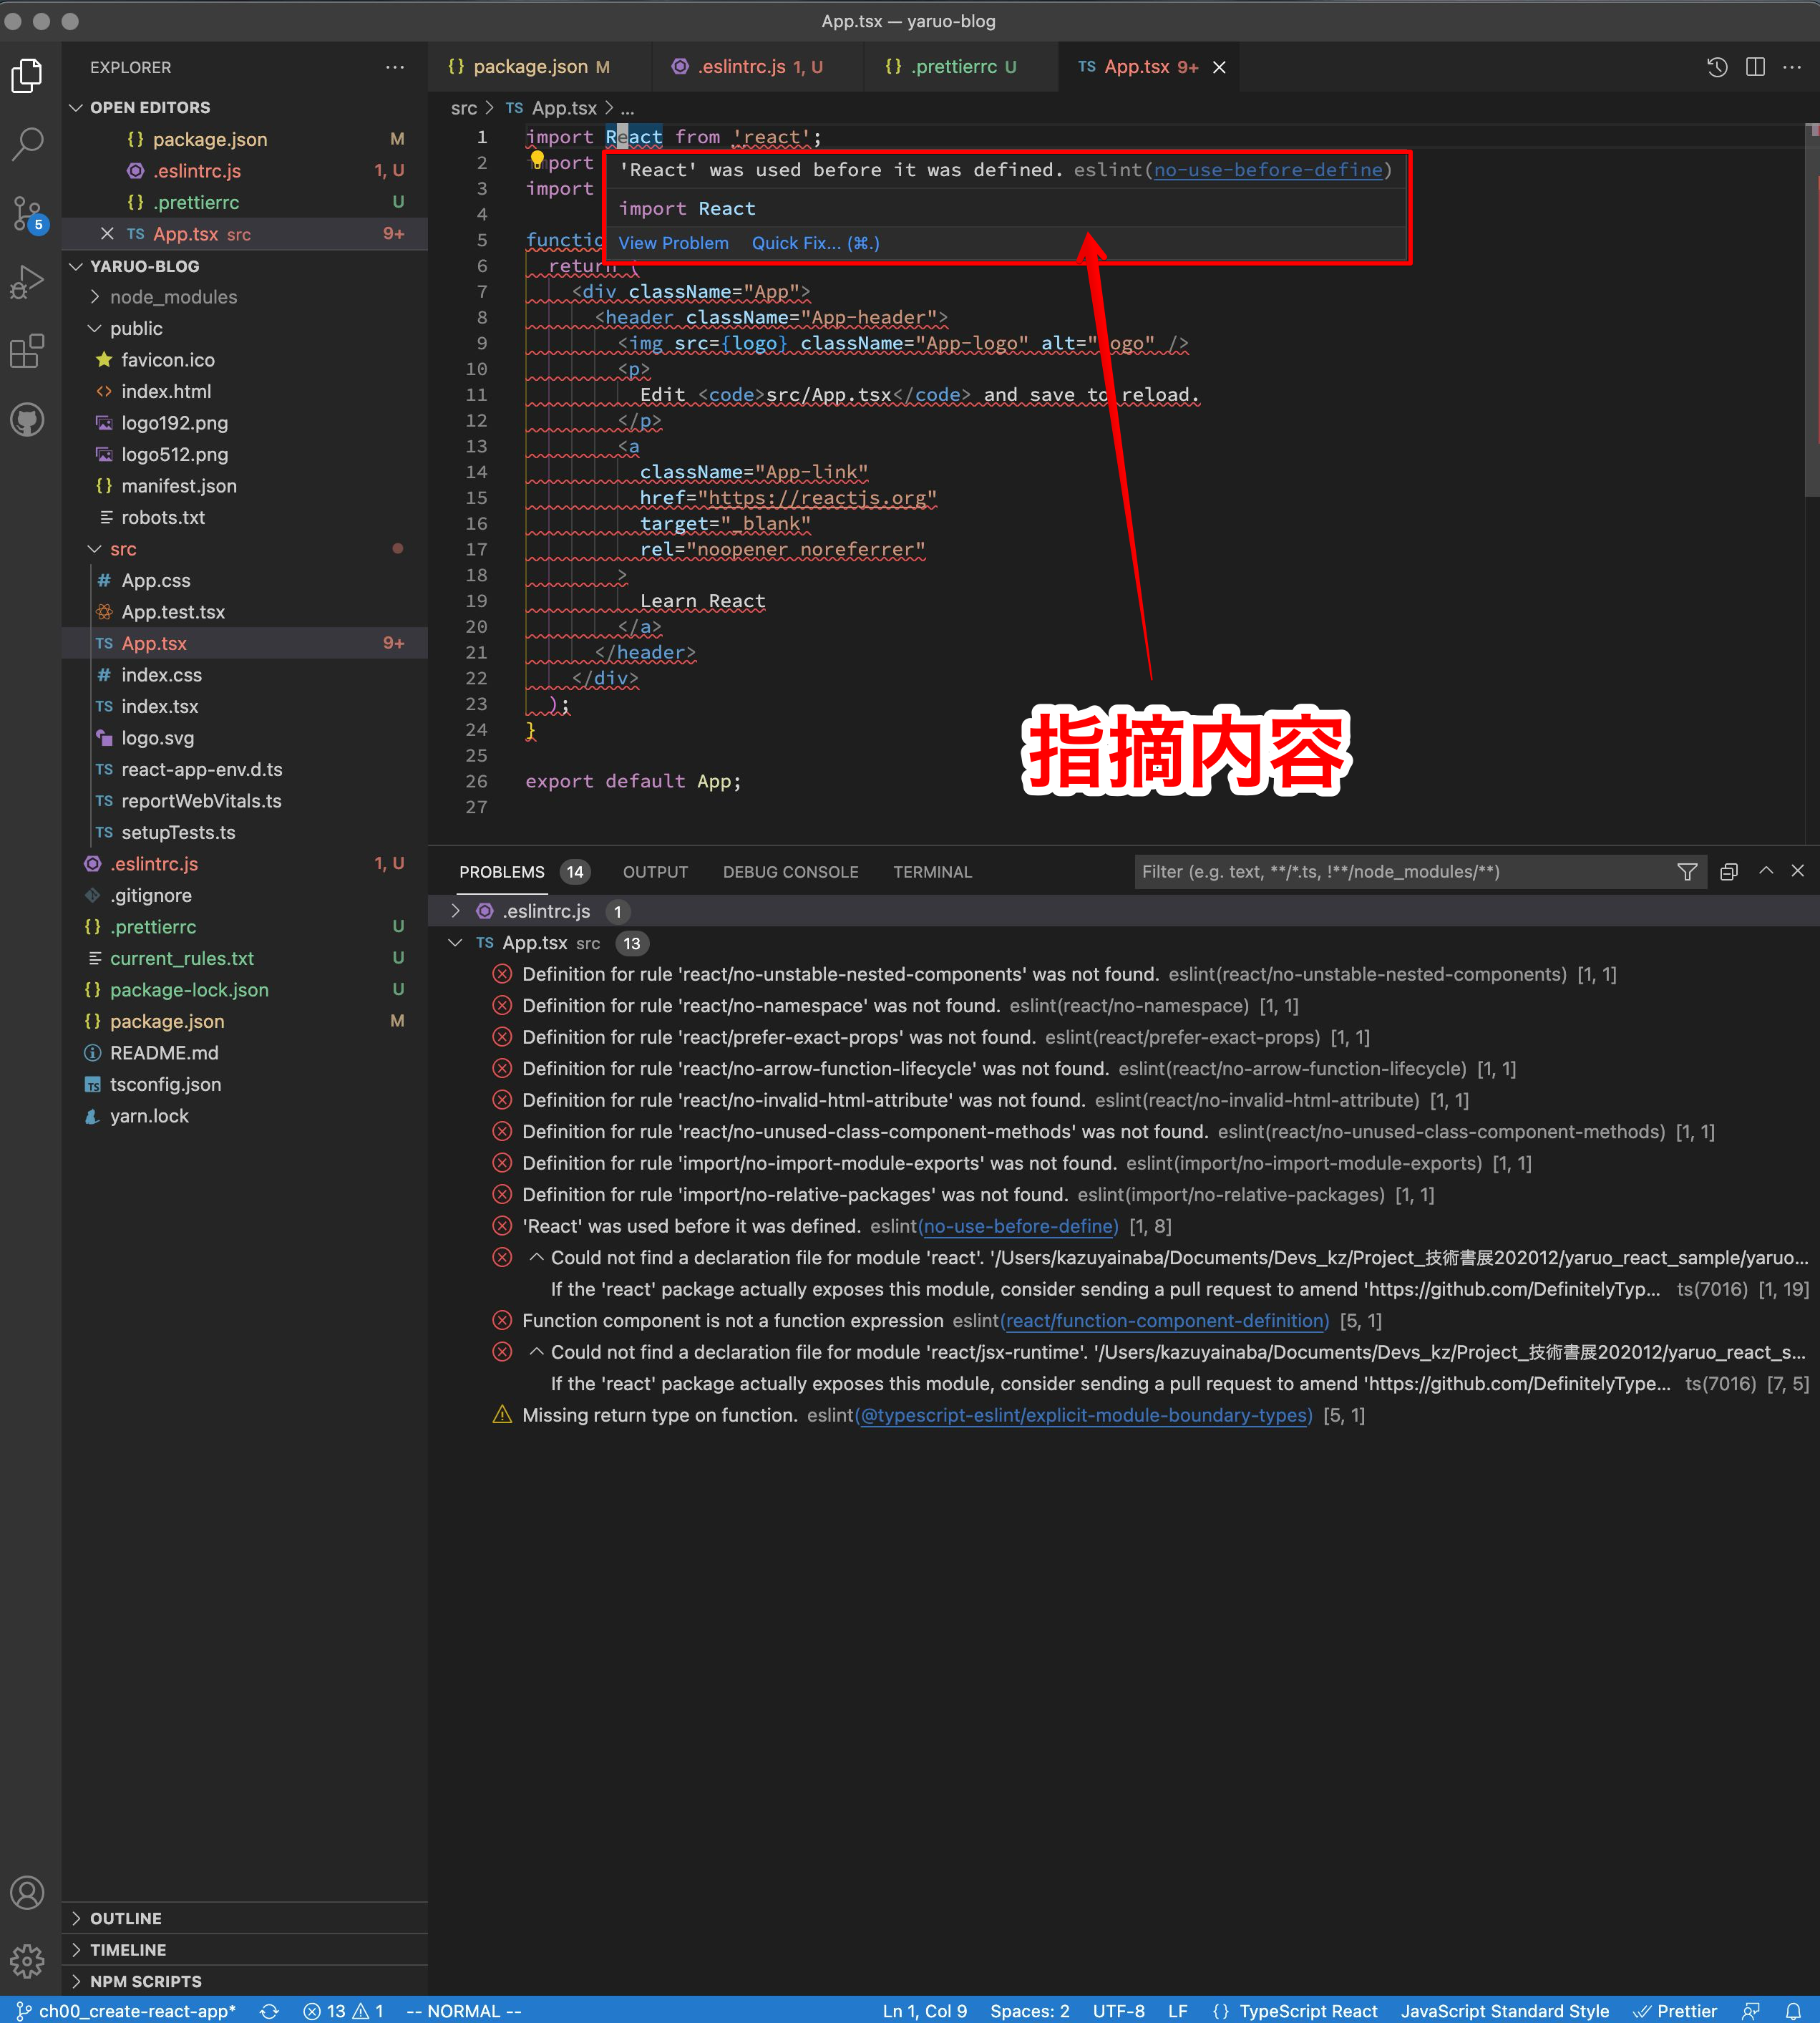
\includegraphics[width=1.0\maxwidth]{./images/02-create-react-app/04_eslint_prettier_fix.png}%
\reviewimagecaption{ポップアップが表示}
\label{image:02-create-react-app:04_eslint_prettier_fix}
\end{reviewimage}
\begin{starternote}[]{}

筆者がVSCodeを日本語化していないのは、エラーメッセージでググる場合を考えてのことです。
英語でのエラーメッセージの方が的確なページをみつけやすいと考えています。

\end{starternote}

では、指摘されている点を修正していきます。

\def\startercodeblockfontsize{}
\begin{starterprogram}[]{App.tsx}\seqsplit{  // React17からは、JSXでReactのインポートが不要になりましたので、以下の行を削除します。
  import React from 'react';}\end{starterprogram}
\def\startercodeblockfontsize{}
\begin{starterprogram}[]{App.tsx}\seqsplit{  import React, \{ ReactElement \} from "react";
  import logo from "./logo.svg";
  import "./App.css";

  const App = (): ReactElement =\textgreater{} \{
    return (
      \textless{}div className="App"\textgreater{}}\end{starterprogram}

このように、戻り値の型を指定することで指摘を修正できました。

\begin{reviewimage}[H]%%06_eslint_prettier_fixdoneAll
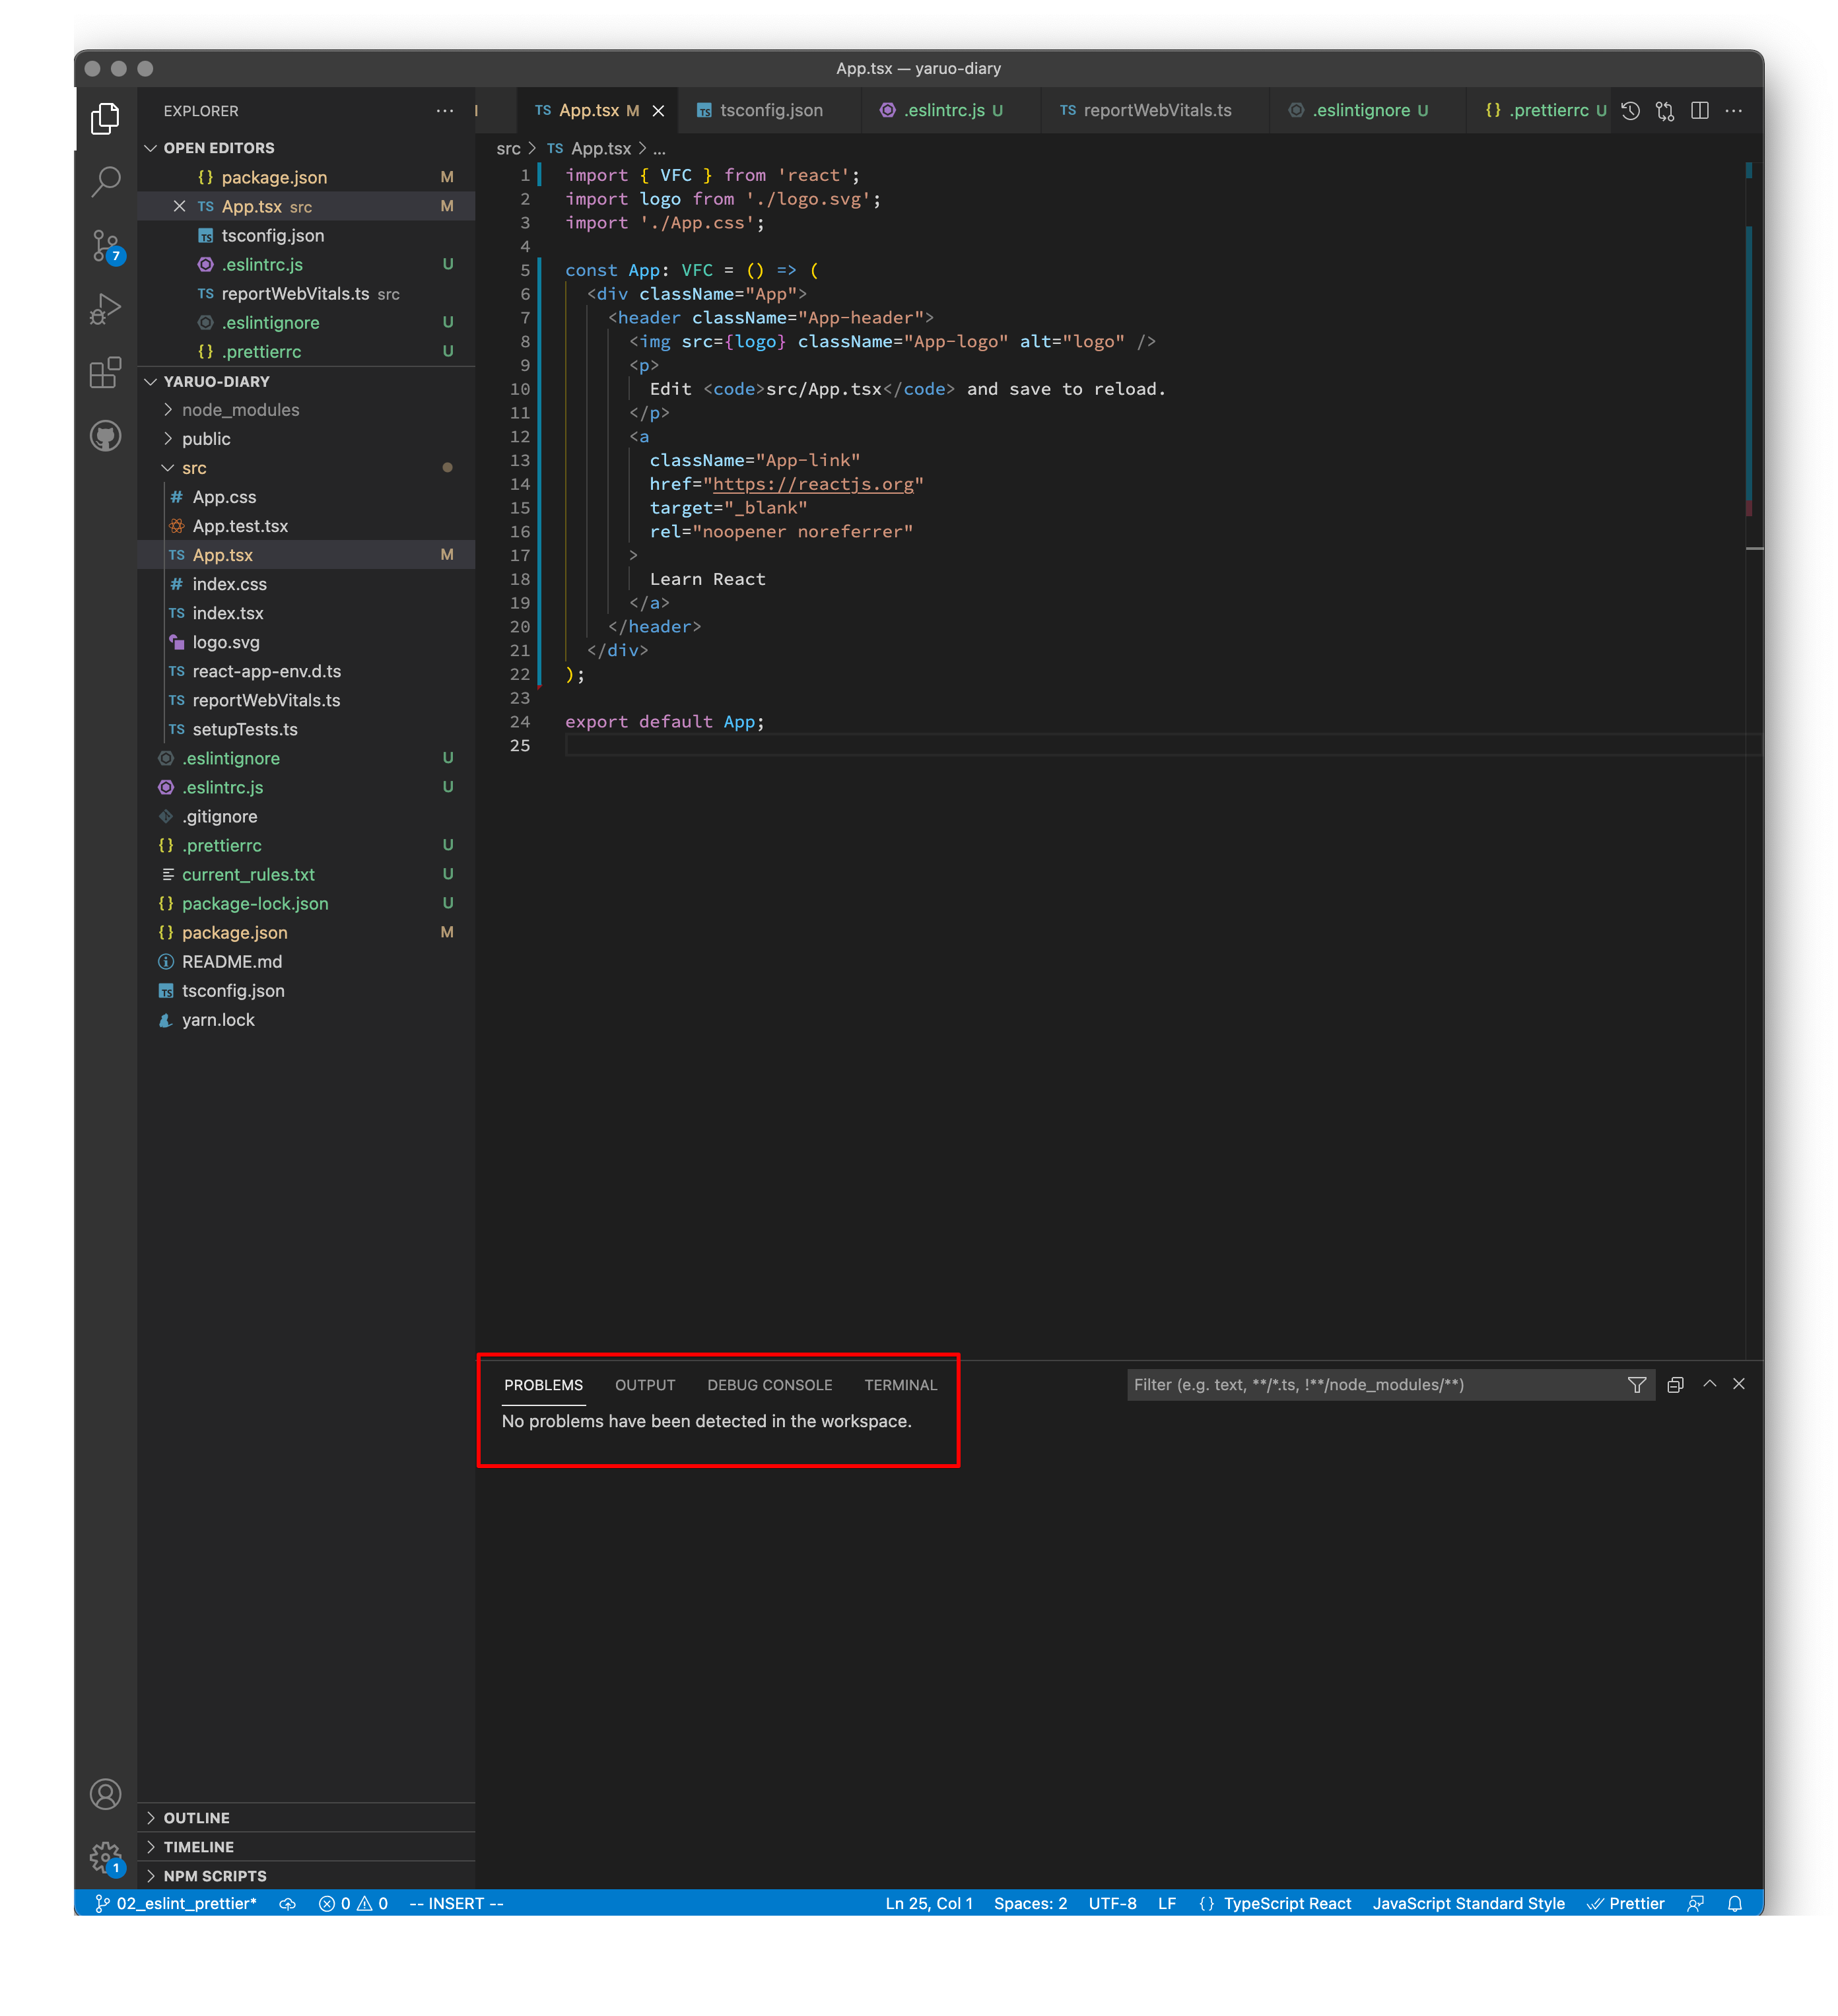
\includegraphics[width=1.0\maxwidth]{./images/02-create-react-app/06_eslint_prettier_fixdoneAll.png}%
\reviewimagecaption{すべての問題の修正完了}
\label{image:02-create-react-app:06_eslint_prettier_fixdoneAll}
\end{reviewimage}

\section{第2章のまとめ}
\keeplastskip{
  \label{sec:2-6}
  \label{sec-chap02review}
  \par\nobreak
}

Reactを使用したアプリケーションは、スタートアップ用のアプリケーションがコマンド一発でインストールできます。

より良いコーディングをするためにも、Eslint、Prettierを導入しましょう。

\begin{starternote}[]{}

ここまでの内容は、GitHub上で、以下のコマンドでクローンできます。
\textless{}!{-}{-} textlint{-}disable {-}{-}\textgreater{}

\def\startercodeblockfontsize{}
\begin{starterterminal}[]{GitHub}\seqsplit{  \textdollar{} \textgreater{} git clone {-}b 01\textunderscore{}eslint\textunderscore{}prettier https://github.com/tmkkz/yaruo.git}\end{starterterminal}

\textless{}!{-}{-} textlint{-}enable {-}{-}\textgreater{}

\end{starternote}
